\documentclass[border=10pt]{standalone}
\usepackage{tikz}
\usepackage{pgfplots}
\pgfplotsset{compat=1.17}

\begin{document}
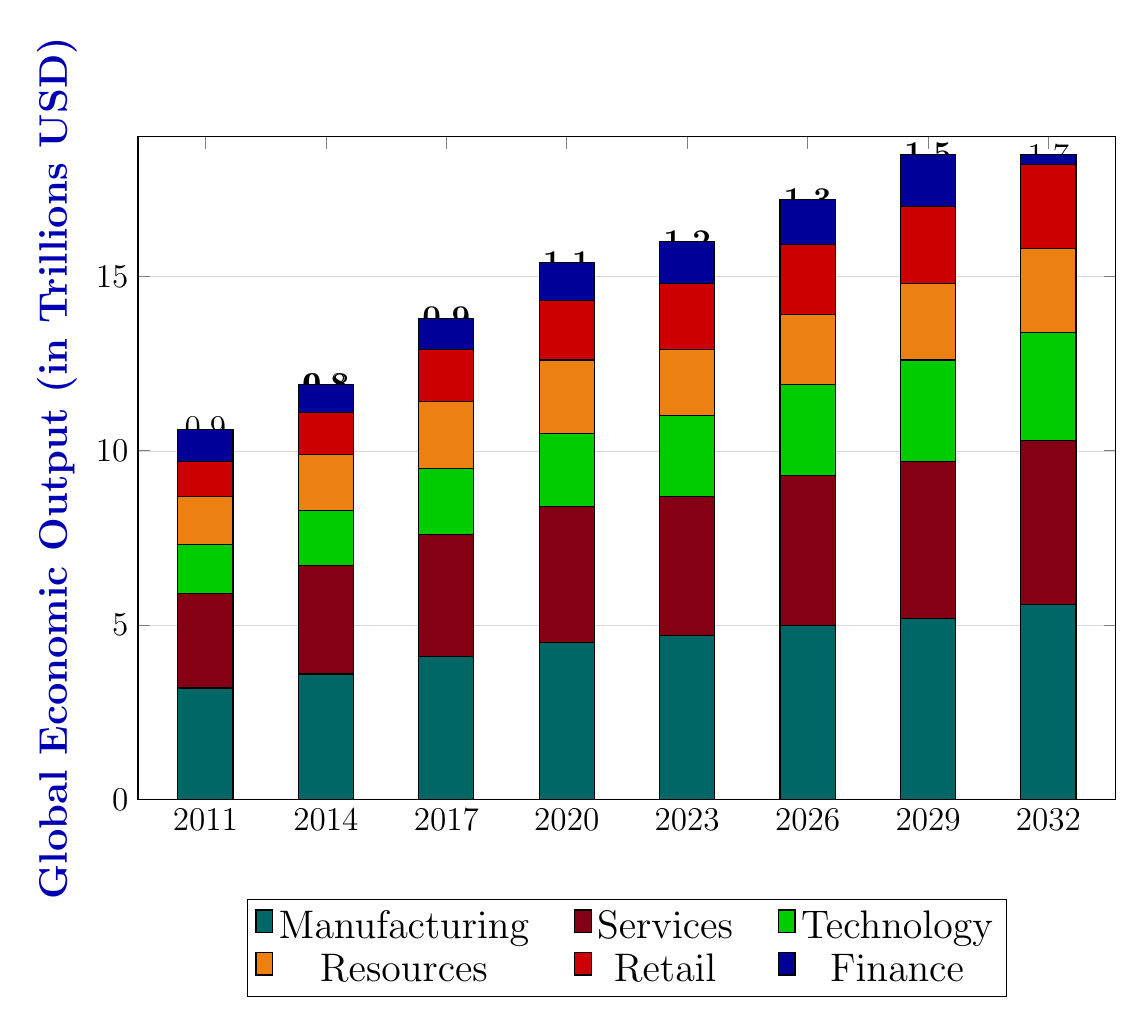
\begin{tikzpicture}
\begin{axis}[
    ybar stacked,
    width=14cm,
    height=10cm,
    bar width=0.7cm,
    ylabel={Global Economic Output (in Trillions USD)},
    ylabel style={font=\Large\bfseries, color=blue!70!black},
    ymin=0,
    ymax=19,
    ytick={0,5,10,15},
    xtick=data,
    xticklabels={2011, 2014, 2017, 2020, 2023, 2026, 2029, 2032},
    xticklabel style={font=\large},
    yticklabel style={font=\large},
    legend style={
        at={(0.5,-0.15)},
        anchor=north,
        legend columns=3,
        font=\Large,
        /tikz/every even column/.append style={column sep=0.5cm}
    },
    ymajorgrids=true,
    grid style={line width=0.1pt, draw=gray!30},
    enlarge x limits=0.08,
    nodes near coords style={font=\large, text=white},
]

% Manufacturing (teal)
\addplot[fill=teal!80!black, draw=black] coordinates {
    (1,3.2) (2,3.6) (3,4.1) (4,4.5) (5,4.7) (6,5.0) (7,5.2) (8,5.6)
};

% Services (burgundy)
\addplot[fill=purple!50!red!60!black, draw=black] coordinates {
    (1,2.7) (2,3.1) (3,3.5) (4,3.9) (5,4.0) (6,4.3) (7,4.5) (8,4.7)
};

% Technology (green)
\addplot[fill=green!80!black, draw=black] coordinates {
    (1,1.4) (2,1.6) (3,1.9) (4,2.1) (5,2.3) (6,2.6) (7,2.9) (8,3.1)
};

% Resources (brown/orange)
\addplot[fill=orange!70!brown, draw=black] coordinates {
    (1,1.4) (2,1.6) (3,1.9) (4,2.1) (5,1.9) (6,2.0) (7,2.2) (8,2.4)
};

% Retail (red)
\addplot[fill=red!80!black, draw=black] coordinates {
    (1,1.0) (2,1.2) (3,1.5) (4,1.7) (5,1.9) (6,2.0) (7,2.2) (8,2.4)
};

% Finance (blue)
\addplot[fill=blue!60!black, draw=black] coordinates {
    (1,0.9) (2,0.8) (3,0.9) (4,1.1) (5,1.2) (6,1.3) (7,1.5) (8,0.3)
};

% Add total labels on top of bars
\node[font=\large\bfseries] at (axis cs:1,10.2) {0.6};
\node[font=\large\bfseries] at (axis cs:2,11.9) {0.8};
\node[font=\large\bfseries] at (axis cs:3,13.8) {0.9};
\node[font=\large\bfseries] at (axis cs:4,15.4) {1.1};
\node[font=\large\bfseries] at (axis cs:5,16.0) {1.2};
\node[font=\large\bfseries] at (axis cs:6,17.2) {1.3};
\node[font=\large\bfseries] at (axis cs:7,18.5) {1.5};

% Add segment value labels
% 2011
\node[font=\large] at (axis cs:1,1.6) {3.2};
\node[font=\large] at (axis cs:1,4.55) {2.7};
\node[font=\large] at (axis cs:1,6.6) {1.4};
\node[font=\large] at (axis cs:1,8.3) {1.4};
\node[font=\large] at (axis cs:1,9.6) {1};
\node[font=\large] at (axis cs:1,10.65) {0.9};

% 2014
\node[font=\large] at (axis cs:2,1.8) {3.6};
\node[font=\large] at (axis cs:2,5.15) {3.1};
\node[font=\large] at (axis cs:2,7.5) {1.6};
\node[font=\large] at (axis cs:2,9.3) {1.6};
\node[font=\large] at (axis cs:2,10.7) {1.2};
\node[font=\large] at (axis cs:2,11.9) {0.8};

% 2017
\node[font=\large] at (axis cs:3,2.05) {4.1};
\node[font=\large] at (axis cs:3,5.85) {3.5};
\node[font=\large] at (axis cs:3,8.55) {1.9};
\node[font=\large] at (axis cs:3,10.55) {1.9};
\node[font=\large] at (axis cs:3,12.05) {1.5};
\node[font=\large] at (axis cs:3,13.35) {0.9};

% 2020
\node[font=\large] at (axis cs:4,2.25) {4.5};
\node[font=\large] at (axis cs:4,6.45) {3.9};
\node[font=\large] at (axis cs:4,9.55) {2.1};
\node[font=\large] at (axis cs:4,11.65) {2.1};
\node[font=\large] at (axis cs:4,13.35) {1.7};
\node[font=\large] at (axis cs:4,14.95) {1.1};

% 2023
\node[font=\large] at (axis cs:5,2.35) {4.7};
\node[font=\large] at (axis cs:5,6.7) {4};
\node[font=\large] at (axis cs:5,9.85) {2.3};
\node[font=\large] at (axis cs:5,11.65) {1.9};
\node[font=\large] at (axis cs:5,13.65) {1.9};
\node[font=\large] at (axis cs:5,15.6) {1.2};

% 2026
\node[font=\large] at (axis cs:6,2.5) {5};
\node[font=\large] at (axis cs:6,7.15) {4.3};
\node[font=\large] at (axis cs:6,10.3) {2.6};
\node[font=\large] at (axis cs:6,12.3) {2};
\node[font=\large] at (axis cs:6,14.3) {2};
\node[font=\large] at (axis cs:6,16.55) {1.3};

% 2029
\node[font=\large] at (axis cs:7,2.6) {5.2};
\node[font=\large] at (axis cs:7,7.45) {4.5};
\node[font=\large] at (axis cs:7,10.85) {2.9};
\node[font=\large] at (axis cs:7,12.95) {2.2};
\node[font=\large] at (axis cs:7,15.05) {2.2};
\node[font=\large] at (axis cs:7,17.75) {1.5};

% 2032
\node[font=\large] at (axis cs:8,2.8) {5.6};
\node[font=\large] at (axis cs:8,8.0) {4.7};
\node[font=\large] at (axis cs:8,11.95) {3.1};
\node[font=\large] at (axis cs:8,14.35) {2.4};
\node[font=\large] at (axis cs:8,16.55) {2.4};
\node[font=\large] at (axis cs:8,18.45) {1.7};

\legend{Manufacturing, Services, Technology, Resources, Retail, Finance}

\end{axis}
\end{tikzpicture}
\end{document}